\documentclass[11pt,a4paper]{article}
\usepackage[utf8]{inputenc}
\usepackage[T1]{fontenc}
\usepackage[french]{babel}
\usepackage{lmodern}
\usepackage{amsmath,amssymb}
\usepackage{bm}
\usepackage{booktabs,array}
\usepackage{graphicx}
\usepackage{tikz}
\usepackage[margin=2.5cm]{geometry}
\usepackage{hyperref}

\newcommand{\vm}{\bm{m}}
\newcommand{\vs}{\bm{s}}
\newcommand{\ee}{\mathrm{e}}
\emergencystretch=3em

\title{Injection de spin à travers un empilement polariseur :\\
  le cas test unidimensionnel de Valet et Fert}
\author{}
\date{\today}

\begin{document}

\maketitle

\begin{abstract}
  Ce document accompagne le cas de validation
  \texttt{validation/valet\_fert\_1d} de la branche \texttt{slonczewski}
  de FeeLLGood. Il explique le modèle de Valet et Fert (modèle à deux
  courants avec diffusion de spin), les hypothèses du cas test, l'équation
  résolue et sa solution analytique, la façon dont FeeLLGood résout le
  même problème (empilement polariseur non maillé, condition de Robin sur
  la surface d'entrée), et les résultats attendus. Les dérivations sont
  faites en entier ; un résultat simple en ressort : la polarisation du
  courant injecté est la moyenne des polarisations des éléments de
  l'empilement pondérée par leurs résistances de spin.
\end{abstract}

\tableofcontents

\section{Objet du test}

Dans la branche \texttt{slonczewski}, le courant polarisé n'est plus
injecté avec une polarisation imposée. Le polariseur F1, l'espaceur N et
les deux interfaces F1/N et N/F2 ne sont pas maillés : ils sont éliminés
analytiquement et remplacés par une condition de Robin sur la surface
d'entrée de l'échantillon F2 (clé \texttt{slonczewski} d'une région de
surface, \texttt{src/slonczewskiInterface.h},
\texttt{spinAcc::stackBoundaryCondition}).

Le test vérifie cette condition sur le cas le plus simple où une solution
exacte existe : un fil, des aimantations colinéaires, un courant uniforme.
Le problème est alors celui que Valet et Fert ont résolu en 1993 pour la
magnétorésistance géante en courant perpendiculaire (CPP-GMR). Il contrôle
en particulier :
\begin{itemize}
  \item la conversion, faite par FeeLLGood, des paramètres d'interface de
    la littérature ($AR^*$ en $\Omega\,$m$^2$, asymétrie $\gamma$) en
    conductances du problème de diffusion de spin ;
  \item la renormalisation par le volume de F1 (épaisseur finie, réservoir
    de l'autre côté) ;
  \item l'élimination du nœud espaceur ;
  \item l'équivalence entre les équations de volume de FeeLLGood (diffusion
    anisotrope de Zhang--Levy--Fert avec $\beta=\beta'=P$) et celles de
    Valet--Fert.
\end{itemize}
Les termes transverses (conductance de mélange $G_{\uparrow\downarrow}$,
précession s--d) ne jouent aucun rôle ici : ils sont validés par le cas
\texttt{validation/slonczewski\_angle}.

\section{Le modèle de Valet et Fert}

\subsection{Hypothèses}

\begin{enumerate}
  \item \textbf{Régime diffusif.} Le libre parcours moyen $\lambda$ est
    petit devant la longueur de diffusion de spin $l_{sf}$ : on peut
    remplacer l'équation de Boltzmann par des équations de dérive--diffusion
    pour des potentiels électrochimiques. Valet et Fert ont montré que
    c'est la limite exacte de Boltzmann quand $\lambda\ll l_{sf}$.
  \item \textbf{Deux courants.} Les électrons de moment majoritaire ($+$,
    moment parallèle à l'aimantation) et minoritaire ($-$) conduisent en
    parallèle, avec leurs conductivités $\sigma_\pm$ et leurs potentiels
    électrochimiques $\mu_\pm$. Ils ne se mélangent que par renversement de
    spin (\emph{spin flip}), plus lent que les autres collisions.
  \item \textbf{Colinéarité.} Toutes les aimantations sont parallèles ou
    antiparallèles à un même axe $z$. L'accumulation de spin est alors un
    scalaire (sa composante sur $z$) et les conductances de mélange
    n'interviennent pas.
  \item \textbf{Réponse linéaire, régime stationnaire.} Les écarts à
    l'équilibre sont proportionnels au courant ; on cherche l'état
    stationnaire.
  \item \textbf{Une dimension.} Le courant est uniforme et perpendiculaire
    aux couches ; tout dépend de la seule coordonnée $x$ le long de
    l'empilement.
  \item \textbf{Interfaces minces.} Une interface est une couche d'épaisseur
    nulle qui conserve le spin, caractérisée par des résistances par unité
    de surface dépendant du spin, $r_\pm = 2AR^*(1\mp\gamma)$. Il n'y a pas
    de perte de mémoire de spin à l'interface.
  \item \textbf{Réservoirs.} Loin de l'empilement (contacts), les électrons
    sont à l'équilibre : l'accumulation de spin y est nulle.
\end{enumerate}

\subsection{Loi d'Ohm à deux courants}

On prend ici $e>0$ (charge élémentaire). Pour chaque canal, la densité de
courant de charge $j_\pm$ suit la loi d'Ohm généralisée
\begin{equation}
  j_\pm = \frac{\sigma_\pm}{e}\,\frac{d\mu_\pm}{dx},
  \qquad
  \sigma_\pm = \frac{\sigma}{2}\,(1\pm\beta),
  \label{eq:ohm}
\end{equation}
où $\sigma$ est la conductivité totale et $\beta$ la polarisation en
volume, $0\le\beta<1$ ($\beta = P$ dans FeeLLGood). Les électrons
descendent le gradient de $\mu_\pm$ ; le courant de charge, de sens
opposé, le remonte. On introduit le potentiel moyen et l'accumulation de
spin, exprimée en volts :
\begin{equation}
  \bar\mu = \frac{\mu_++\mu_-}{2},
  \qquad
  \varphi = \frac{\mu_+-\mu_-}{2e},
  \qquad
  \mu_\pm = \bar\mu \pm e\varphi .
\end{equation}
Le courant total $j = j_++j_-$ et le courant de spin $j_s = j_+-j_-$
(exprimé comme un courant de charge) valent
\begin{equation}
  j = \frac{\sigma}{e}\,\bar\mu' + \sigma\beta\,\varphi',
  \qquad
  j_s = \frac{\sigma\beta}{e}\,\bar\mu' + \sigma\,\varphi' .
\end{equation}
En éliminant $\bar\mu'$ entre les deux :
\begin{equation}
  \boxed{\;j_s = \beta\,j + \sigma(1-\beta^2)\,\varphi'\;}
  \label{eq:js-volume}
\end{equation}
Le premier terme est le courant de spin \og de dérive\fg{} : loin de toute
interface, une fraction $\beta$ du courant est polarisée. Le second est un
courant de diffusion, avec la conductivité de spin $\sigma(1-\beta^2) =
1/\rho^*$ (notation de Valet--Fert, $\rho^* = \rho/(1-\beta^2)$).

\subsection{Équation de diffusion}

La charge est conservée, $j' = 0$ : $j$ est uniforme. Le spin ne l'est
pas : les renversements de spin font relaxer $\varphi$, et
\begin{equation}
  j_s' = \frac{\sigma(1-\beta^2)}{l_{sf}^2}\,\varphi .
\end{equation}
Cette relation définit la longueur de diffusion de spin $l_{sf}$ (notée
$l_{sf}^*$ par Baltz).
Avec \eqref{eq:js-volume} et $j' = 0$, on obtient l'équation de Valet et
Fert :
\begin{equation}
  \boxed{\;\varphi'' = \frac{\varphi}{l_{sf}^2}\;}
  \label{eq:diffusion}
\end{equation}
Dans chaque couche, $\varphi$ est une combinaison de
$\ee^{x/l_{sf}}$ et $\ee^{-x/l_{sf}}$ : l'accumulation de spin naît aux
interfaces et s'amortit sur $l_{sf}$ de part et d'autre.

\paragraph{Remarque : $l_{sf}$ et les longueurs par canal.} Valet et Fert
écrivent $1/l_{sf}^2 = 1/l_{sf,+}^2 + 1/l_{sf,-}^2$, où
$l_{sf,\pm} = \sqrt{D_\pm\tau_\pm}$ fait intervenir le temps $\tau_\pm$ au
bout duquel \emph{un} électron du canal $\pm$ renverse son spin. Il n'y a
pas de facteur 2 : l'écart $\mu_+-\mu_-$ diminue aussi bien quand un $+$
devient $-$ que quand un $-$ devient $+$, et les deux taux s'ajoutent comme
des conductances en parallèle. Dans un métal normal, $l_{sf,+} = l_{sf,-} =
l_0$ donne $l_{sf} = l_0/\sqrt2$ : l'accumulation relaxe deux fois plus vite
qu'un électron isolé ne renverse son spin. $l_{sf}$ n'est donc pas une
moyenne des $l_{sf,\pm}$ ; il est plus petit que chacune d'elles. C'est la
seule longueur mesurable (longueur de décroissance de $\varphi$, tirée par
exemple de la CPP-GMR), et c'est elle que FeeLLGood prend comme paramètre
(\texttt{l\_sf}) ; les $l_{sf,\pm}$ n'y interviennent pas.

\subsection{Conditions d'interface}

À une interface de résistances $r_\pm = 2AR^*(1\mp\gamma)$, chaque canal
traverse une résistance, et $\mu_\pm$ saute :
$j_\pm = \Delta\mu_\pm/(e\,r_\pm)$, avec $\Delta\mu_\pm = \Delta\bar\mu \pm
e\,\Delta\varphi$ (saut de droite moins gauche). Avec
$1/r_\pm = (1\pm\gamma)/\left(2AR^*(1-\gamma^2)\right)$ :
\begin{equation}
  j = \frac{\Delta\bar\mu/e + \gamma\,\Delta\varphi}{AR^*(1-\gamma^2)},
  \qquad
  j_s = \frac{\gamma\,\Delta\bar\mu/e + \Delta\varphi}{AR^*(1-\gamma^2)} .
\end{equation}
En éliminant $\Delta\bar\mu$, on obtient la loi d'interface, de même
forme que \eqref{eq:js-volume} :
\begin{equation}
  \boxed{\;j_s = \gamma\,j + \frac{\Delta\varphi}{AR^*}\;}
  \label{eq:js-interface}
\end{equation}
$\gamma$ joue pour l'interface le rôle de $\beta$ pour le volume, et
$AR^*$ celui de la résistance de spin. Les courants $j$ et $j_s$ sont
continus à travers l'interface (pas de perte de spin).

\subsection{Un cadre commun : la résistance de spin}

Les relations \eqref{eq:js-volume} et \eqref{eq:js-interface} ont la
même structure. Pour un élément $k$ de l'empilement (volume ou
interface), le courant de spin qui le traverse s'écrit
\begin{equation}
  j_s = P_k\,j + \frac{\Delta\varphi_k}{r_k},
  \label{eq:element}
\end{equation}
où $P_k$ est sa polarisation, $r_k$ sa résistance de spin (en
$\Omega\,$m$^2$) et $\Delta\varphi_k$ la variation de $\varphi$ à travers lui (droite moins gauche).
C'est un générateur de Norton : une source de courant $P_kj$ en parallèle
sur une résistance $r_k$. Les couches de volume s'y ramènent quand le courant de
spin y est conservé à leur bord, ce qui est le cas des deux couches du
test (section~\ref{sec:circuit}).

\section{Le cas test}

\subsection{Géométrie}

\begin{figure}[h]
\centering
\begin{tikzpicture}[x=1cm,y=1cm]
  \fill[blue!12] (0,0) rectangle (3,1.4);
  \fill[gray!25] (3,0) rectangle (3.25,1.4);
  \fill[red!10] (3.25,0) rectangle (12,1.4);
  \draw (0,0) rectangle (12,1.4);
  \draw[thick] (3,0) -- (3,1.4);
  \draw[thick] (3.25,0) -- (3.25,1.4);
  \node at (1.5,0.95) {F1};
  \node at (1.5,0.45) {$t_1$, $\beta_1$, $l_{sf,1}$};
  \node at (7.6,0.95) {F2 (maillé)};
  \node at (7.6,0.45) {$L$, $\beta_2$, $l_{sf,2}$};
  \draw[->,thick] (0.6,1.75) -- (1.4,1.75) node[right] {$\pm\bm{p}$};
  \draw[->,thick] (6.8,1.75) -- (7.6,1.75) node[right] {$\vm$};
  \node[below] at (0,0) {$x=-t_1$};
  \node[below] at (3.1,0) {$x=0$};
  \node[below] at (12,0) {$x=L$};
  \node[above] at (3.12,1.4) {\small N};
  \draw[<-] (2.95,-0.75) -- (2.2,-1.2) node[left] {\small F1/N : $AR_1^*$, $\gamma_1$};
  \draw[<-] (3.3,-0.75) -- (4.1,-1.2) node[right] {\small N/F2 : $AR_2^*$, $\gamma_2$};
  \node[left] at (0,0.7) {\small réservoir};
  \node[right] at (12,0.7) {\small réservoir};
  \draw[->,very thick] (4.5,-0.45) -- (6.5,-0.45) node[right] {\small électrons};
\end{tikzpicture}
\caption{L'empilement. Seul F2 est maillé ; F1, l'espaceur N (d'épaisseur
  nulle) et les deux interfaces sont éliminés analytiquement. Les
  électrons vont de F1 vers F2.}
\label{fig:empilement}
\end{figure}

L'empilement est représenté figure~\ref{fig:empilement}. L'axe $x$ du
modèle est l'axe $z$ du maillage. L'échantillon F2 est un fil de section
$10\times10$\,nm$^2$ et de longueur $L = 300$\,nm (\texttt{wire.geo},
taille de maille $h = 1$\,nm, 30\,607 nœuds, tétraèdres P1). Ses faces
latérales ne laissent passer ni charge ni spin (condition de Neumann
nulle) : le problème reste unidimensionnel. Les aimantations sont selon
$z$ : F2 vers $+z$, F1 vers $+z$ (configuration P) ou $-z$ (AP). En AP,
$\beta_1$ et $\gamma_1$ changent de signe.

\subsection{Paramètres}

\begin{center}
\renewcommand{\arraystretch}{1.2}
\begin{tabular}{llll}
  \toprule
  Élément & Paramètre & Valeur & Clé FeeLLGood \\
  \midrule
  F2 (fil) & $\sigma_2$ & $4\times10^6$\,S/m & \texttt{sigma} \\
    & $\beta_2$ & 0.3 & \texttt{P} \\
    & $l_{sf,2}$ & 10\,nm & \texttt{l\_sf} \\
    & $l_{sd}$ & 1\,nm & \texttt{l\_sd} \\
    & $N_0$ & $1.344\times10^{47}$\,J$^{-1}$m$^{-3}$ & \texttt{dens\_state} \\
  F1 & $\sigma_1$ & $2\times10^6$\,S/m & \texttt{F1.sigma} \\
    & $\beta_1$ & 0.5 & \texttt{F1.P} \\
    & $l_{sf,1}$ & 20\,nm & \texttt{F1.l\_sf} \\
    & $t_1$ & 15\,nm & \texttt{F1.thickness} \\
  F1/N & $AR_1^*$, $\gamma_1$ & $0.5\times10^{-15}\,\Omega\,$m$^2$, 0.75
    & \texttt{F1N.AR}, \texttt{F1N.gamma} \\
  N/F2 & $AR_2^*$, $\gamma_2$ & $0.3\times10^{-15}\,\Omega\,$m$^2$, 0.6
    & \texttt{NF2.AR}, \texttt{NF2.gamma} \\
  Courant & $j_n$ & $10^{12}$\,A/m$^2$ & \texttt{jn} (entrée) \\
  \bottomrule
\end{tabular}
\end{center}

La normale sortante de la surface d'entrée est $-z$ ; $j_n = \bm{J}\cdot
\bm{n} > 0$ signifie que le courant de charge sort de F2 par l'entrée,
donc que les électrons y entrent. Le courant de charge le long de $x$ vaut
$j = -j_n$. Les conductances de mélange (\texttt{Gr} $= 5\times10^{14}$\,S/m$^2$)
sont données mais n'interviennent pas.

\subsection{Conditions aux limites}

\begin{itemize}
  \item $x = -t_1$ (réservoir derrière F1) : $\varphi = 0$ ;
  \item $x = L$ (sortie, réservoir) : $\varphi = 0$ et $V = 0$
    (\texttt{outlet}: \texttt{V: 0}, \texttt{s: [0,0,0]}) ;
  \item $x = 0$ : interfaces F1/N et N/F2 de part et d'autre de N, avec
    \eqref{eq:js-interface}, et continuité de $j_s$ à travers N.
\end{itemize}

\section{Solution analytique}

\subsection{Le système linéaire}

On écrit, avec $\ee_1 = \ee^{-t_1/l_{sf,1}}$ et $\ee_2 = \ee^{-L/l_{sf,2}}$,
\begin{align}
  \varphi_1(x) &= a_1\,\ee^{x/l_{sf,1}} + d_1\,\ee^{-(x+t_1)/l_{sf,1}},
    & -t_1 &\le x\le 0, \\
  \varphi_2(x) &= a_2\,\ee^{-x/l_{sf,2}} + d_2\,\ee^{(x-L)/l_{sf,2}},
    & 0 &\le x\le L,
\end{align}
et $\varphi_N$ l'accumulation dans l'espaceur. Les cinq inconnues
$(a_1, d_1, \varphi_N, a_2, d_2)$ sont fixées par :
\begin{enumerate}
  \item $\varphi_1(-t_1) = 0$ ;
  \item $\varphi_2(L) = 0$ ;
  \item le courant de spin sortant de F1 en $x=0^-$, donné par
    \eqref{eq:js-volume}, est celui de l'interface F1/N :
    $\beta_1 j + c_1\varphi_1'(0) = \gamma_1 j + (\varphi_N-\varphi_1(0))/AR_1^*$ ;
  \item il traverse l'espaceur :
    $\gamma_1 j + (\varphi_N-\varphi_1(0))/AR_1^* =
     \gamma_2 j + (\varphi_2(0)-\varphi_N)/AR_2^*$ ;
  \item il entre dans F2 :
    $\gamma_2 j + (\varphi_2(0)-\varphi_N)/AR_2^* = \beta_2 j + c_2\varphi_2'(0)$,
\end{enumerate}
avec $c_k = \sigma_k(1-\beta_k^2)$. C'est le système $5\times5$ résolu par
la fonction \texttt{valet\_fert} du script. On en tire
l'accumulation de spin de FeeLLGood (section~\ref{sec:conversion}) :
$s_z(x) = \mu_B N_0\,e\,\varphi_2(x)/2$.

\subsection{Lecture en circuit : la polarisation injectée}
\label{sec:circuit}

Le système se résout aussi à la main, et la solution s'interprète
simplement. Comme $L = 30\,l_{sf,2}$, on peut prendre F2 semi-infini
($\ee_2 \simeq 10^{-13}$) : $\varphi_2(x) = \varphi_2(0)\,\ee^{-x/l_{sf,2}}$,
donc $\varphi_2'(0) = -\varphi_2(0)/l_{sf,2}$ et
\begin{equation}
  j_s(0^+) = \beta_2\,j + \frac{0-\varphi_2(0)}{r_2},
  \qquad r_2 = \frac{l_{sf,2}}{\sigma_2(1-\beta_2^2)} = \rho_2^*\,l_{sf,2} .
\end{equation}
F2 est l'élément \eqref{eq:element} de polarisation $\beta_2$ et de
résistance de spin $r_2$, la chute $\varphi$ allant de $\varphi_2(0)$ à
0 au loin. De même, dans F1, $\varphi_1(x) = \varphi_1(0)\sinh\left((x+t_1)/l_{sf,1}\right)/
\sinh(t_1/l_{sf,1})$, donc
\begin{equation}
  j_s(0^-) = \beta_1\,j + \frac{\varphi_1(0)-0}{R_1},
  \qquad R_1 = \rho_1^*\,l_{sf,1}\tanh\frac{t_1}{l_{sf,1}} .
\end{equation}
La résistance de spin d'une couche d'épaisseur finie posée sur un
réservoir est réduite par $\tanh(t_1/l_{sf,1})$ : c'est l'inverse de la
conductance $g_F$ de la note \texttt{slonczewski\_polarisation.tex}.

Le courant de spin $j_s$ est le même dans les quatre éléments (F1,
F1/N, N/F2, F2), et les chutes de $\varphi$ s'ajoutent de 0 (réservoir
de F1) à 0 (loin dans F2). En sommant \eqref{eq:element},
$\sum_k (j_s - P_kj)\,r_k = 0$, d'où
\begin{equation}
  \boxed{\;\frac{j_s}{j} = P_{\mathrm{inj}}
  = \frac{\beta_1R_1 + \gamma_1AR_1^* + \gamma_2AR_2^* + \beta_2r_2}
         {R_1 + AR_1^* + AR_2^* + r_2}\;}
  \label{eq:Pinj}
\end{equation}
\textbf{La polarisation du courant injecté est la moyenne des
polarisations des éléments, pondérée par leurs résistances de spin.} Un
élément de grande résistance de spin impose sa polarisation ; c'est
l'origine du désaccord d'impédance (une couche de résistance de spin
énorme, comme un semiconducteur, impose $P_{\mathrm{inj}}\simeq0$).

L'accumulation à l'entrée de F2 s'en déduit :
\begin{equation}
  \boxed{\;\varphi_2(0) = (P_{\mathrm{inj}}-\beta_2)\,j_n\,r_2\;}
  \label{eq:phi0}
\end{equation}
(avec $j = -j_n$). Le signe de $s$ à l'entrée dit si F2 reçoit plus de
spin majoritaire qu'il ne sait en transporter en volume
($P_{\mathrm{inj}} > \beta_2$, $s>0$) ou moins ($s<0$).

\subsection{Valeurs numériques}

Les résistances de spin valent
\begin{center}
\begin{tabular}{lcc}
  \toprule
  Élément & $r_k$ ($10^{-15}\,\Omega\,$m$^2$) & $P_k$ (P / AP) \\
  \midrule
  F1, $R_1 = \rho_1^*l_{sf,1}\tanh(t_1/l_{sf,1})$ & 8.469 & $+0.5$ / $-0.5$ \\
  F1/N, $AR_1^*$ & 0.5 & $+0.75$ / $-0.75$ \\
  N/F2, $AR_2^*$ & 0.3 & 0.6 \\
  F2, $r_2 = \rho_2^*l_{sf,2}$ & 2.747 & 0.3 \\
  \midrule
  Total & 12.016 & \\
  \bottomrule
\end{tabular}
\end{center}
et \eqref{eq:Pinj} donne
\begin{center}
\renewcommand{\arraystretch}{1.2}
\begin{tabular}{lccc}
  \toprule
  & $P_{\mathrm{inj}}$ & $\varphi_2(0)$ (mV) & $s_z(0)$ (A/m) \\
  \midrule
  P  & $+0.467$ & $+0.459$ & $+45.86$ \\
  AP & $-0.300$ & $-1.648$ & $-164.60$ \\
  \bottomrule
\end{tabular}
\end{center}
Le rapport AP/P vaut $(-0.300-0.3)/(0.467-0.3) = -3.59$. Ces valeurs
sont celles de la résolution exacte du système $5\times5$ (l'écart dû à
F2 fini est de l'ordre de $\ee^{-30}$).

\textbf{Interprétation.} En P, F1 et l'interface F1/N, très polarisés,
injectent un courant plus polarisé ($0.467$) que celui que F2 transporte
en volume ($0.3$) : des électrons majoritaires s'accumulent à l'entrée,
$s>0$. En AP, F1 polarise le courant à contre-sens ; malgré l'interface
N/F2 et F2 qui tirent vers $+0.6$ et $+0.3$, le courant injecté est
polarisé à $-0.30$. L'écart à $\beta_2$ est 3.6 fois plus grand : les
minoritaires s'accumulent, $s<0$, et plus fortement. Dans les deux cas,
$s$ décroît en $\ee^{-x/l_{sf,2}}$ : à $x = 10$\,nm, il vaut $1/\ee$ de sa
valeur d'entrée (16.87\,A/m en P). La différence des chutes de potentiel
entre P et AP est la CPP-GMR.

\section{Ce que résout FeeLLGood}

\subsection{Équations de volume}
\label{sec:conversion}

FeeLLGood résout pour l'accumulation de spin $\vs$ (en A/m)
\begin{equation}
  \nabla\cdot Q = -\frac{\vs}{\tau_{sf}} - \frac{\vs\times\vm}{\tau_{sd}},
  \qquad
  Q_{i\alpha} = -P\,\frac{\mu_B}{e}\,j_i\,m_\alpha
  - D_0\left[\partial_i s_\alpha - P^2 m_\alpha(\vm\cdot\partial_i\vs)\right],
\end{equation}
avec $D_0 = 2\sigma/(e^2N_0)$ et, dans les régions magnétiques,
$1/\tau_{sf} = D_0(1-P^2)/l_{sf}^2$. Dans le cas colinéaire,
$\vs = s\,\vm$ et $\vs\times\vm = 0$ ; la diffusion le long de $\vm$ vaut
$D_0(1-P^2)$ et le flux de moment le long de $x$ est
\begin{equation}
  Q = -P\,\frac{\mu_B}{e}\,j - D_0(1-P^2)\,s' .
\end{equation}
Avec $s = \mu_BN_0e\varphi/2$ et $D_0 = 2\sigma/(e^2N_0)$, on a
$D_0(1-P^2)\,s' = (\mu_B/e)\,\sigma(1-P^2)\,\varphi'$, donc
\begin{equation}
  Q = -\frac{\mu_B}{e}\left[P\,j + \sigma(1-P^2)\,\varphi'\right]
    = -\frac{\mu_B}{e}\,j_s :
\end{equation}
le courant de FeeLLGood est exactement $-(\mu_B/e)$ fois le courant de spin
\eqref{eq:js-volume} de Valet--Fert, avec $\beta = P$. L'équation de
relaxation donne de même $s'' = s/l_{sf}^2$, c'est-à-dire
\eqref{eq:diffusion}. Le facteur $1/2$ de la conversion vient de ce que
$D_0$ vaut deux fois le coefficient $D$ de la relation d'Einstein
$\sigma = e^2N_0D$ : $\vs$ est la moitié de l'aimantation physique
$\mu_BN_0\mu_s$, ce qui ne change aucun résultat.

Cette équivalence demande la diffusion anisotrope : la clé
\texttt{anisotropic\_diffusion} de la section \texttt{spin\_accumulation}
doit valoir \texttt{true}, ce qui est la valeur par défaut. Sans elle, la conductivité de spin de F2 serait $\sigma$ au lieu
de $\sigma(1-P^2)$ et le test échouerait.

\subsection{La condition de Robin sur l'entrée}

L'empilement non maillé (F1, F1/N, N, N/F2) est la mise en série des trois
premiers éléments de \eqref{eq:element}. En sommant leurs chutes de
$\varphi$ entre le réservoir de F1 et l'entrée de F2 :
\begin{equation}
  j_s = P_{\mathrm{st}}\,j + \frac{\varphi_2(0)}{R_{\mathrm{st}}},
  \qquad
  R_{\mathrm{st}} = R_1 + AR_1^* + AR_2^*,
  \qquad
  P_{\mathrm{st}} = \frac{\beta_1R_1 + \gamma_1AR_1^* + \gamma_2AR_2^*}{R_{\mathrm{st}}} .
\end{equation}
Converti en flux de moment entrant dans F2 avec $s = \mu_BN_0e\varphi/2$
et $j = -j_n$, c'est la condition de Robin
\begin{equation}
  \boxed{\;q = \frac{\mu_B}{e}\,j_n\,P_{\mathrm{st}} - G\,s,
  \qquad G = \frac{k}{R_{\mathrm{st}}},\quad k = \frac{2}{e^2N_0}\;}
\end{equation}
($G$ en m/s). C'est ce que construit FeeLLGood dans le cas colinéaire :
\begin{itemize}
  \item \texttt{Slonczewski::makeStack} convertit chaque interface,
    $G_\parallel = k/AR^*$ et $P = \gamma$ ;
  \item \texttt{renormalizeF1} met en série le volume de F1, de
    conductance $g_F = k/R_1 = k\,\sigma_1(1-\beta_1^2)\coth(t_1/l_{sf,1})/l_{sf,1}$,
    avec la conductance de F1/N :
    \[
      G_{\parallel1}^* = \frac{g_FG_{\parallel1}}{g_F+G_{\parallel1}},
      \qquad
      P_1^* = \frac{\beta_1g_F + \gamma_1G_{\parallel1}}{g_F+G_{\parallel1}} ;
    \]
  \item \texttt{effectiveBC} élimine le nœud espaceur : la conductance
    effective est la mise en série $G_2(G_1+G_2)^{-1}G_1$, la polarisation
    effective la moyenne pondérée correspondante.
\end{itemize}
Les conductances sont toutes converties avec la densité d'états $N_0$ de
F2, la région de volume qui borde la surface : celle de F1 n'intervient
pas.

Le problème discret est le problème de diffusion de FeeLLGood sur le fil
avec cette condition sur l'entrée et $\vs = 0$ sur la sortie. Comme la
condition de Robin est exacte pour l'empilement non maillé, la seule
erreur est celle de la discrétisation de F2.

\section{Résultats attendus}

\subsection{Profils}

\begin{figure}[h]
\centering
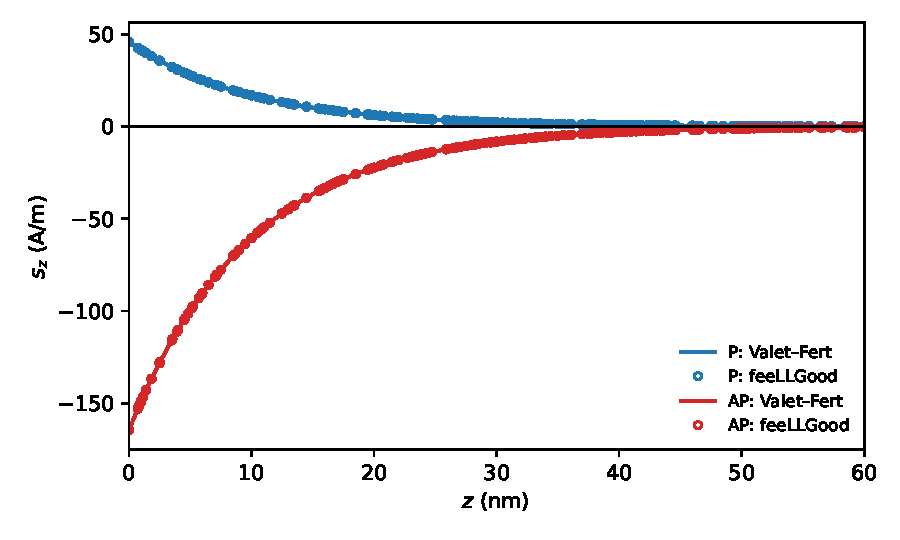
\includegraphics[width=0.8\textwidth]{valet_fert_1d_profile.pdf}
\caption{Accumulation de spin $s_z$ le long du fil : solution de
  Valet--Fert (traits) et valeurs de FeeLLGood en 250 nœuds tirés au
  hasard (cercles), configurations P et AP, $h = 1$\,nm. Seuls les 60
  premiers nanomètres sont montrés ; au-delà, $s_z$ est nul.}
\label{fig:profil}
\end{figure}

La figure~\ref{fig:profil} compare les deux solutions. Les nœuds d'une
même abscisse ont la même valeur à la précision du graphique : la solution
est bien unidimensionnelle, et ses composantes transverses $s_x$, $s_y$
sont nulles (elles valent exactement 0 dans les fichiers \texttt{.sol}).

\subsection{Précision et convergence}

Le script compare $s_z$ aux nœuds à la solution analytique et calcule
l'erreur maximale rapportée à $\max|s_z|$ :
\begin{center}
\renewcommand{\arraystretch}{1.2}
\begin{tabular}{lccc}
  \toprule
  Maillage & P : $s_z(0)$ FeeLLGood / VF & AP : $s_z(0)$ FeeLLGood / VF
    & erreur max \\
  \midrule
  $h = 2$\,nm & 45.690 / 45.858\,A/m & $-163.994$ / $-164.596$\,A/m
    & $8.2\times10^{-3}$ \\
  $h = 1$\,nm & 45.811 / 45.858\,A/m & $-164.427$ / $-164.596$\,A/m
    & $2.6\times10^{-3}$ \\
  \bottomrule
\end{tabular}
\end{center}
L'erreur décroît comme $h^2$, ce qu'on attend d'éléments P1 pour une
solution régulière. Elle est la même en P et en AP : rapportée à
$\max|s_z|$, elle ne dépend que du rapport $h/l_{sf,2}$ (ici $1/10$) et
de la condition de Robin, qui a la même forme dans les deux cas. Le temps
de calcul est d'environ 25\,s pour les deux configurations.

\subsection{Ce que le test détecte}

\begin{itemize}
  \item \textbf{Facteur de conversion.} Avec $G_\parallel = 1/(e^2N_0AR^*)$
    au lieu de $2/(e^2N_0AR^*)$, l'erreur passe à 8.5\,\% en P : le test
    échoue (tolérance 1\,\%).
  \item \textbf{Renormalisation de F1.} Oublier le volume de F1
    ($R_1 = 0$) change $P_{\mathrm{inj}}$ de 0.467 à 0.389 en P
    (formule~\eqref{eq:Pinj}) : d'après \eqref{eq:phi0}, $s_z(0)$ est
    presque divisé par 2.
  \item \textbf{Diffusion isotrope.} Avec
    \texttt{anisotropic\_diffusion: false}, F2 n'a plus les équations de
    Valet--Fert : l'erreur passe à 7.3\,\% en P et le test échoue.
\end{itemize}

\subsection{Utilisation}

\begin{verbatim}
cd validation/valet_fert_1d
./valet_fert.py [chemin de feellgood]     # défaut : ../../src/feellgood
\end{verbatim}
Le maillage est construit par \texttt{gmsh} s'il manque. Le script
écrit les réglages de chaque configuration, lance FeeLLGood sur une durée
très courte (le problème de diffusion de spin est stationnaire et résolu
à chaque pas), lit les fichiers \texttt{P\_iter0.sol} et
\texttt{AP\_iter0.sol}, et affiche :
\begin{verbatim}
P : s_z(inlet) feeLLGood =    45.811 A/m, Valet-Fert =    45.858 A/m;
    max error / max|s| = 2.63e-03, transverse = 0.0e+00
AP: s_z(inlet) feeLLGood =  -164.427 A/m, Valet-Fert =  -164.596 A/m;
    max error / max|s| = 2.63e-03, transverse = 0.0e+00
OK
\end{verbatim}
Le code de retour est 0 si l'erreur est inférieure à 1\,\% dans les deux
configurations.

\section{Limites du test}

\begin{itemize}
  \item Le test est colinéaire : il ne dit rien des conductances de
    mélange, de la précession s--d, ni du choix \texttt{sink} ou
    \texttt{series} pour la partie transverse. Le cas
    \texttt{validation/slonczewski\_angle} les couvre.
  \item F2 est une seule région : la continuité de $\vs$ entre deux
    régions maillées de densités d'états différentes est testée par
    \texttt{validation/two\_regions\_1d}.
  \item Le modèle de Valet--Fert ne contient pas de perte de mémoire de
    spin aux interfaces ; FeeLLGood non plus.
  \item Le maillage résout largement $l_{sf,2} = 10$\,nm. Dans un vrai
    calcul, il faut aussi résoudre la longueur transverse
    $l_{sd}\sim1$\,nm, ce que ce test ne vérifie pas.
\end{itemize}

\section*{Références}

\begin{itemize}
  \item T.~Valet, A.~Fert, \emph{Theory of the perpendicular
    magnetoresistance in magnetic multilayers}, Phys.\ Rev.\ B
    \textbf{48}, 7099 (1993).
  \item S.~Zhang, P.\,M.~Levy, A.~Fert, Phys.\ Rev.\ Lett.\ \textbf{88},
    236601 (2002) : diffusion de spin non colinéaire.
  \item A.~Fert, H.~Jaffrès, Phys.\ Rev.\ B \textbf{64}, 184420 (2001) :
    injection de spin et désaccord d'impédance.
  \item V.~Baltz, \emph{The Basics of Electron Transport in Spintronics},
    EDP Sciences (2023), §3.2--3.4 et exercice 6.3.
  \item \texttt{dev-notes/slonczewski\_polarisation.tex} : dérivation de
    la condition de Robin, renormalisation de F1, conversion des
    conductances.
  \item \texttt{dev-notes/spin\_injection\_boundary\_conditions.md} (en
    anglais) : la même, avec la mise en œuvre dans FeeLLGood.
\end{itemize}

\end{document}
